\chapter{Anhang }
\label{cha:Anhang}

\section{GDBMS-Implementierungen}
\label{anh:vendor_list}

\renewcommand{\arraystretch}{1.25}
\begin{table}[h]
	\centering
	\begin{footnotesize}
   	\begin{tabular}{|m{2.5cm}|m{3.5cm}|>{\arraybackslash}m{9.25cm}|}
	\hline	
	\textbf{GDBMS} & \textbf{Hersteller} & \textbf{Website} \\
	\hline
   	Affinity 		& GoPivotal 			& \url{http://affinityng.cfapps.io/} \\
   	ArangoDB 		& triAGENS 				& \url{http://www.arangodb.org/} \\
   	Bitsy 			& Privatperson 			& \url{https://bitbucket.org/lambdazen/bitsy/} \\
   	DEX 			& Sparsity Technologies & \url{http://www.sparsity-technologies.com/dex} \\
   	Filament 		& Privatperson 			& \url{http://sourceforge.net/projects/filament/} \\
   	FlockDB 		& Twitter				& \url{https://github.com/twitter/flockdb} \\
   	GraphBase 		& FactNexus 			& \url{http://graphbase.net/} \\
   	GraphPack 		& Privatperson 			& \url{https://code.google.com/p/graphpack/} \\
   	G-Store 		& Forschungsprototyp	& \url{http://g-store.sourceforge.net/} \\
   	Horton 			& Microsoft 			& \url{http://research.microsoft.com/en-us/projects/ldg/} \\
   	HyperGraphDB 	& Kobrix Software		& \url{http://www.hypergraphdb.org/index} \\
   	InfiniteGraph 	& Objectivity			& \url{http://www.objectivity.com/infinitegraph} \\
   	Fallen-8 		& Privatperson 			& \url{http://www.fallen-8.com/} \\
   	Neo4j 			& Neo Technology 		& \url{http://www.neo4j.org/} \\
   	OQGRAPH 		& Open Query 			& \url{http://openquery.com/node/23} \\
   	OrientDB 		& Orient Technologies 	& \url{http://www.orientdb.org/} \\
   	RedisGraph 		& Privatperson 			& \url{https://github.com/tblobaum/redis-graph} \\
   	SGDB3 			& Forschungsprototyp 	& \url{http://ups.savba.sk/~marek/sgdb.html} \\
   	Titan 			& Aurelius 				& \url{http://thinkaurelius.github.io/titan/} \\
   	Trinity 		& Microsoft 			& \url{http://research.microsoft.com/en-us/projects/trinity/} \\
   	VertexDB 		& Privatperson 			& \url{https://github.com/stevedekorte/vertexdb} \\
   	\hline
   	\end{tabular} 
	\end{footnotesize}
	\setlength{\belowcaptionskip}{0.25cm}	
	\caption[GDBMS-Hersteller]{Liste der Webseiten untersuchter GDBMS.}
	\label{tab:anh_urls}
\end{table}
\renewcommand{\arraystretch}{1}

\section{Quelltextbeispiele}

Abbildung \ref{fig:example} zeigt einen Property-Graphen, auf den sich die nachfolgenden Quelltextbeispiele beziehen. Die Attribute und Bezeichner der Knoten und Kanten entsprechen denen im Benchmark. Die Beispiele zeigen die Syntax f�r das Erzeugen von Knoten- und Kanteninstanzen, das Auslesen der Nachbarschaft eines Knotens sowie - wenn vorhanden - die Verwendung von Traversal Frameworks und mengenorientierten APIs.

\begin{figure}[h] 
	\centering
		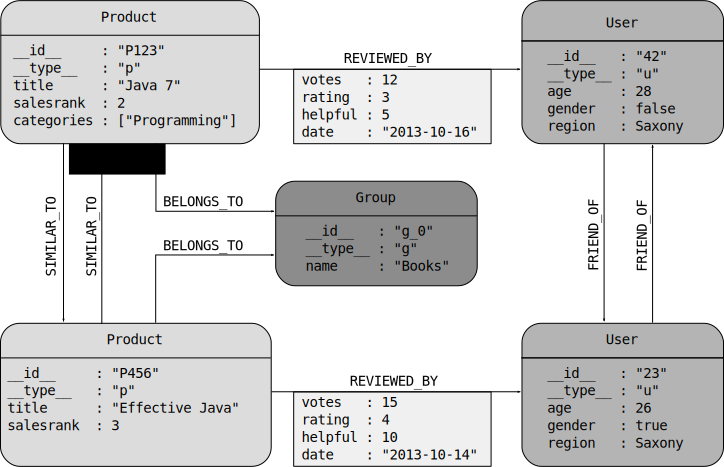
\includegraphics[scale=.75]{example.pdf}
	\caption[Anhang: Beispielgraph]{Datengrundlage f�r Quellcodebeispiele.}
	\label{fig:example}
\end{figure}

\newpage

\subsection*{Neo4j}
\label{anh:neo4j_api}

\lstset{language=Java, basicstyle=\ttfamily\footnotesize, caption={Neo4j: CRUD-Operationen}, label=list:neo4j_api_example}
\begin{lstlisting}
try (Transaction tx = graphDB.beginTx()) {
	// create labels
	Label productLabel = new Label() {@Override public String name() { 
		return "Product"; }};
	Label userLabel = new Label() {@Override public String name() {
	    return "User";
	}};
	// ...
	
	// create a product node instance
	Node p123 = graphDB.createNode(productLabel); // no __type__ attribut needed
	p123.setProperty("__id__", "p123");
	p123.setProperty("title", "Effective Java");
	p123.setProperty("salesrank", 2);
	p123.setProperty("categories", new String[] { "Programming" });
	// create a user node instance
	Node u42 = graphDB.createNode(userLabel);
	u42.setProperty("__id__", "u42");
	u42.setProperty("age", 28);
	u42.setProperty("gender", false);
	u42.setProperty("region", "Saxony");
	// ...
	
	// create REVIEWED_BY edge instance
	Relationship review1 = p123.createRelationshipTo(u42, 
		RelTypes.REVIEWED_BY); // edge label has been defined before
	review1.setProperty("votes", 12);
	review1.setProperty("rating", 3);
	review1.setProperty("helpful", 5);
	review1.setProperty("date", "2013-10-06");
	// ...
	
	// make changes persistent
	tx.success();
	
	// read the neighbourhood of p123 using all outgoing edges
	for (Relationship e : p123.getRelationships(Direction.OUTGOING)) {
		System.out.println(e.getType().name() + " points to "
			+ e.getEndNode().getProperty("__id__"));
	}
	// prints ...
	// SIMILAR_TO points to p456
	// BELONGS_TO points to g0
	// REVIEWED_BY points to u42
}
\end{lstlisting}

\lstset{language=Java, basicstyle=\ttfamily\footnotesize, caption={Neo4j: Traversal Framework}, label=list:neo4j_traversal_example}
\begin{lstlisting}
// abstract path description
TraversalDescription td = Traversal.description()
	// traverse the graph in breadth first order
	.breadthFirst()
	// consider the following edge labels and directions
	.relationships(RelTypes.FRIEND_OF, Direction.INCOMING)
	.relationships(RelTypes.REVIEWED_BY, Direction.BOTH)
	.relationships(RelTypes.SIMILAR_TO, Direction.OUTGOING)
	// no zero length paths
	.evaluator(Evaluators.excludeStartPosition());
	
// start traversal at user u23
for (Path p : td.traverse(u23)) {
	System.out.println(p);
}
// prints paths ...
// (5)<--[FRIEND_OF,4]--(4) // 4 => u42
// (5)<--[REVIEWED_BY,7]--(3) // 3 => p456
// (5)<--[FRIEND_OF,4]--(4)<--[REVIEWED_BY,6]--(2) // 2 => p123
\end{lstlisting}

\subsection*{HypergraphDB}

\lstset{language=Java, basicstyle=\ttfamily\footnotesize, caption={HyperGraphDB: CRUD-Operationen}, label=list:hgdb_api_example}
\begin{lstlisting}
// create JavaBean instances
Group books = new Group(1L, "Books");
Product p123 = new Product("p123", "Java 7", 2, new String[] { "Programming" });
Product p456 = new Product("p456", "Effective Java", 3, null);
User u42 = new User("u42", 28, false, "Saxony");
User u23 = new User("u23", 26, true, "Saxony");
Review rev1 = new Review("2013-10-16", 3, 12, 5);
Review rev2 = new Review("2013-10-14", 4, 15, 10);

// create atom handles for the nodes
HGHandle booksHandle = hg.add(books);
HGHandle p123Handle = hg.add(p123);
HGHandle p456Handle = hg.add(p456);
HGHandle u42Handle = hg.add(u42);
HGHandle u23Handle = hg.add(u23);

// link atoms using their handles
hg.add(new HGRel("belongs_to", p123Handle, booksHandle));
hg.add(new HGRel("belongs_to", p456Handle, booksHandle));
hg.add(new HGRel("similar_to", p123Handle, p456Handle));
hg.add(new HGRel("similar_to", p456Handle, p123Handle));
hg.add(new HGRel("friend_of", u42Handle, u23Handle));
hg.add(new HGRel("friend_of", u23Handle, u42Handle));
// use HGValueLink to store a value at the edge
hg.add(new HGValueLink(rev1, p123Handle, u42Handle));
hg.add(new HGValueLink(rev2, p456Handle, u23Handle));
\end{lstlisting}

\lstset{language=Java, basicstyle=\ttfamily\footnotesize, caption={HyperGraphDB: Mengenorientierte API}, label=list:hgdb_query_example}
\begin{lstlisting}
// get all products with a salesrank greater than or equal to 3
// load the whole result into a list (instead of using an iterator)
List<Product> = hg.getAll(graph,
	hg.and(hg.type(Product.class), hg.gte("salesrank", 3));
	
// go through the result
for (Product p : products) {
	System.out.println(p);
}
// prints products ...
// Product [__id__=p456, title=Effective Java, salesrank=3, categories=null]
\end{lstlisting}

\lstset{language=Java, basicstyle=\ttfamily\footnotesize, caption={HyperGraphDB: Traversal Framework}, label=list:hgdb_traversal_example}
\begin{lstlisting}
// get product handle
HGHandle p123Handle = graph.getHandle(p123);

// define an adjacency list generator
DefaultALGenerator alGen = new DefaultALGenerator(graph, hg.and(
	// link predicate: traverse reviews which were helpful for at least 5 people
	hg.type(Review.class), hg.gte("helpful", 5)),
	// sibling predicate: just look at users who are at least 25 years old
	hg.and(hg.type(User.class), hg.gte("age", 25)));

// initialize the traversal framework
HGTraversal traversal = new HGBreadthFirstTraversal(p123Handle, alGen);

// start the traversal
while (traversal.hasNext()) {
	Pair<HGHandle, HGHandle> next = traversal.next();
	HGLink link = (HGLink) graph.get(next.getFirst());
	Object atom = graph.get(next.getSecond());
	System.out.println("at atom " + atom + " using link " + link);
}
// prints ...
// at atom User [__id__=u42, age=28, gender=false, region=Saxony] 
// using link Review [date=2013-10-16, rating=3, votes=12, helpful=5]
\end{lstlisting}

\subsection*{OrientDB}

\lstset{language=Java, basicstyle=\ttfamily\footnotesize, caption={OrientDB: CRUD-Operationen}, label=list:orientdb_api_example}
\begin{lstlisting}
// create class for product
OClass product = graph.createVertexType("Product");
// define product attributes and constraints
product.createProperty("__id__", OType.STRING).setMandatory(true).setNotNull(true);
product.createProperty("title", OType.STRING).setMandatory(true);
product.createProperty("salesrank", OType.INTEGER);
product.createProperty("categories", OType.EMBEDDEDLIST, OType.STRING);
// create unique index on __id__ for class product
graph.createKeyIndex("__id__", Vertex.class, new Parameter("type", "UNIQUE"), 
	new Parameter("class", "Product"));

// create class for user
OClass user = graph.createVertexType("User");
user.createProperty("__id__", OType.STRING).setMandatory(true)
	.setNotNull(true);
user.createProperty("age", OType.INTEGER).setMin("0").setMax("90");
user.createProperty("gender", OType.BOOLEAN);
user.createProperty("region", OType.STRING);
// create unique index on __id__ for class user
graph.createKeyIndex("__id__", Vertex.class, new Parameter("type", "UNIQUE"),
	new Parameter("class", "Product"));
// ...

// create class for ReviewedBy edge
OClass reviewedBy = graph.createEdgeType("ReviewedBy");
// create edge attributes and constraints
reviewedBy.createProperty("votes", OType.INTEGER).setMin("0");
reviewedBy.createProperty("rating", OType.INTEGER).setMin("0");
reviewedBy.createProperty("helpful", OType.INTEGER).setMin("0");
reviewedBy.createProperty("date", OType.DATE);
// ...

// create product node instance (define mandatory attributes in constructor)
Vertex p123 = graph.addVertex("class:Product", "__id__", "P123",
		    "title", "Java 7");
p123.setProperty("salesrank", 2);
p123.setProperty("categories", new String[] { "Programming" });
// create user node instance
Vertex u42 = graph.addVertex("class:User", "__id__", "u42");
u42.setProperty("age", 28);
u42.setProperty("gender", false);
u42.setProperty("region", "Saxony");
// ...

// create ReviewedBy edge instance
Edge p123_u42 = graph.addEdge("class:ReviewedBy", p123, u42, null);
p123_u42.setProperty("votes", 12);
p123_u42.setProperty("rating", 3);
p123_u42.setProperty("helpful", 5);
c.set(2013, 10, 16);
p123_u42.setProperty("date", c.getTime());
// ...

// make changes persistent
graph.commit();

// read the neighbourhood of p123 using all outgoing edges
for (Edge e : p123.getEdges(Direction.OUT, new String[] {})) {
	System.out.println(e.getLabel() + " points to "
		+ e.getVertex(Direction.IN).getProperty("__id__"));
}
// prints ...
// SimilarTo points to p456
// BelongsTo points to g0
// ReviewedBy points to u42

// perform an SQL-query
for (Vertex v : (Iterable<Vertex>) graph.command(
	new OCommandSQL("SELECT FROM V WHERE __id__ IS NOT null")).execute()) {
	System.out.println(v.getId() + " (" + v.getProperty("__id__") + ")");
}
// prints ...
// #11:0 (p456)
// #11:1 (p123)
// #12:0 (g0)
// #13:0 (u23)
// #13:1 (u42)
\end{lstlisting}

\subsection*{Titan}

\lstset{language=Java, basicstyle=\ttfamily\footnotesize, caption={Titan: CRUD-Operationen}, label=list:titan_api_example}
\begin{lstlisting}
// create TitanKey for __id__
graphDB.makeType().name("__id__")
	// unique on vertex
	.unique(Direction.BOTH)	
	// create an index for that attribute
	.indexed(Vertex.class)
	.dataType(String.class)
	.makePropertyKey();
	
// create TitanKey for title
graphDB.makeType().name("title")
	.dataType(String.class)
	.unique(Direction.OUT)
	.makePropertyKey();
// ...

// create TitanLabel for BELONGS_TO
graphDB.makeType().name("BELONGS_TO")
	// is unique in outgoing direction
	.unique(Direction.OUT)
	.makeEdgeLabel();
// ...

// create product node instance
Vertex p123 = graphDB.addVertex(null);
p123.setProperty("__id__", "p123");
// store the type because there are no labels / classes
p123.setProperty("__type__", "p");
p123.setProperty("title", "Java 7");
List<String> list = new ArrayList<String>();
list.add("Programming");
p123.setProperty("categories", list);
// create user node instance
Vertex u42 = graphDB.addVertex(null);
u42.setProperty("__id__", "u42");
u42.setProperty("__type__", "u");
u42.setProperty("age", 28);
u42.setProperty("gender", false);
u42.setProperty("region", "Saxony");
// ...

// create REVIEWED_BY edge instance
Edge rev1 = p123.addEdge("REVIEWED_BY", u42);
rev1.setProperty("votes", 12);
rev1.setProperty("rating", 3);
rev1.setProperty("helpful", 5);
rev1.setProperty("date", "2013-10-16");
// ...

// make changes persistent
graphDB.commit();

// read the neighbourhood of p123 using all outgoing edges
// using Blueprints API, so its identical to OrientDB
for (Edge e : p123.getEdges(Direction.OUT, new String[] {})) {
	System.out.println(e.getLabel() + " points to "
		+ e.getVertex(Direction.IN).getProperty("__id__"));
}
// prints ...
// REVIEWED_BY points to u42
// BELONGS_TO points to g0
// SIMILAR_TO points to p456
\end{lstlisting}

\section{Benchmark}

\subsection{Extraktion}
\label{anh:extraction}

\subsection{Operationen}
\label{anh:queries}

% random read
\subsubsection*{\texttt{random\_read}}

\lstset{language=Java, caption={Operation \texttt{random\_read} in Cypher}, label=list:random_read_cypher}
\begin{lstlisting}
START a=node(42) RETURN *;
\end{lstlisting}

\lstset{language=Java, caption={Operation \texttt{random\_read} in Gremlin}, label=list:random_read_gremlin}
\begin{lstlisting}
g.v(42).map();
\end{lstlisting}

% sim products
\subsubsection*{\texttt{sim\_products}}

\lstset{language=Java, caption={Operation \texttt{sim\_products} in Cypher}, label=list:sim_products_cypher}
\begin{lstlisting}
START n=node(42) 
MATCH n-[:SIMILAR_TO*..2]-s 
RETURN DISTINCT s.title AS title;
\end{lstlisting}

\lstset{language=Java, caption={Operation \texttt{sim\_products} in Gremlin}, label=list:sim_products_gremlin}
\begin{lstlisting}
g.v(42).both('SIMILAR_TO').loop(1){it.loops <= 2}.dedup().title;
\end{lstlisting}

% foaf reviews
\subsubsection*{\texttt{foaf\_reviews}}

\lstset{language=Java, caption={Operation \texttt{foaf\_reviews} in Cypher}, label=list:foaf_reviews_cypher}
\begin{lstlisting}
START n=node(42)
MATCH n-[:FRIEND_OF*1..2]-()<-[r:REVIEWED_BY]-p
RETURN p.title AS title, avg(r.rating) AS weight
ORDER BY weight DESC;
\end{lstlisting}

\lstset{language=Java, caption={Operation \texttt{foaf\_reviews} in Gremlin}, label=list:foaf_reviews_gremlin}
\begin{lstlisting}
g.v(42).both('FRIEND_OF').both('FRIEND_OF').inE('REVIEWED_BY')
	.groupBy{it.outV.next().title}{it.rating}{it.sum() * 1.0 / it.size()}
	.cap.orderMap(T.decr);
\end{lstlisting}

% path all
\subsubsection*{\texttt{path\_all}}

\lstset{language=Java, caption={Operation \texttt{path\_all} in Cypher}, label=list:path_all_cypher}
\begin{lstlisting}
START a=node(42), b=node(23) 
MATCH p=a-[:FRIEND_OF|SIMILAR_TO|REVIEWED_BY*..4]-b 
RETURN length(p) AS length, count(p) AS cnt;
\end{lstlisting}

\lstset{language=Java, caption={Operation \texttt{path\_all} in Gremlin}, label=list:path_all_gremlin}
\begin{lstlisting}
a = g.v(42);
b = g.v(23);
visited=[a];
a.both('FRIEND_OF','REVIEWED_BY','SIMILAR_TO')
	.loop(1){it.object != b && it.loops < 5}.retain([b])
	.path._().transform{it.size() - 1}.groupCount().cap();
\end{lstlisting}

% path shortest
\subsubsection*{\texttt{path\_shortest}}

\lstset{language=Java, caption={Operation \texttt{path\_shortest} in Cypher}, label=list:path_shortest_cypher}
\begin{lstlisting}
START a=node(42), b=node(23)
MATCH p=shortestPath(a-[:FRIEND_OF|:REVIEWED_BY|:SIMILAR_TO*..5]-b)
RETURN EXTRACT(n in NODES(p): n.__id__) AS path;
\end{lstlisting}

\lstset{language=Java, caption={Operation \texttt{path\_shortest} in Gremlin}, label=list:path_shortest_gremlin}
\begin{lstlisting}
a = g.v(42);
b = g.v(23);
visited=[a];
a.both('FRIEND_OF', 'REVIEWED_BY', 'SIMILAR_TO')
	.except(visited).store(visited)
	.loop(3){it.object != b && it.loops < 6}.retain([b])
	.path{it.__id__};
\end{lstlisting}

% top regions
\subsubsection*{\texttt{top\_regions}}

\lstset{language=Java, caption={Operation \texttt{top\_region} in Cypher}, label=list:top_region_cypher}
\begin{lstlisting}
START g=node:nodes('__id__':'g0')
MATCH g<-[:BELONGS_TO]-p-[r:REVIEWED_BY]->u
WHERE p.salesrank < 500000
RETURN u.region AS region, count(u) AS cnt
ORDER BY cnt DESC
LIMIT 10;
\end{lstlisting}

\lstset{language=Java, caption={Operation \texttt{top\_region} in Gremlin}, label=list:top_region_gremlin}
\begin{lstlisting}
group = g.V('__id__', 'g0').next();
group.in('BELONGS_TO').filter{it.salesrank < 500000}
	.out('REVIEWED_BY').groupCount{it.region}.cap()
	.orderMap(T.decr)[0..9];
\end{lstlisting}

% sim pattern
\subsubsection*{\texttt{sim\_pattern}}

\lstset{language=Java, caption={Operation \texttt{sim\_pattern} in Cypher}, label=list:sim_pattern_cypher}
\begin{lstlisting}
START user=node(42)
MATCH user-[:FRIEND_OF]-friends1<-[:REVIEWED_BY]-products,
products-[:REVIEWED_BY]->friends2
WITH user, products, collect(distinct friends1.__id__) as f1, collect(distinct friends2.__id__) as f2
WITH user, products, filter(x in f1 : x in f2) as intersect
WITH user, products, count(products) as n, intersect, length(intersect) as intersect_cnt
WHERE intersect_cnt > 1 and n > 0
RETURN user.__id__ as user_id, n, products.__id__ as product_id, intersect as friends, intersect_cnt;
\end{lstlisting}

\lstset{language=Java, caption={Operation \texttt{sim\_pattern} in Gremlin}, label=list:sim_pattern_gremlin}
\begin{lstlisting}
u = g.v(42);
m = [:]; common_products = [] as Set;
u.both("FRIEND_OF").dedup().transform({ it.in("REVIEWED_BY").dedup() })
	.scatter().groupCount(m).filter({ m[it] >= 2 }).fill(common_products);
common_products._().as("product").transform({
	it.out("REVIEWED_BY").filter({
		it.in("REVIEWED_BY").retain(common_products)[0..<2].count() == 2
	}).as("friend").both("FRIEND_OF").retain([u]).back("friend").toSet()
}).as("friends").table().cap().next();
\end{lstlisting}

\section{Zus�tzliche Quellen}

\subsection*{Email-Kommunikation Neo Technology}
\label{anh:mail_neo}

Hi Martin,

It's great to speak with you, thanks for reaching out. Cypher is indeed a great convenience. As you point out, it's not yet always fast: certain operations aren't yet well optimized. There is a good reason for this. Cypher was born right around two years ago: 11 years after the first line of Neo4j code was written, and about a year before Titan was released, for anyone who's counting :-) We have spent a lot of time working on getting the language and functionality right, and not as much time on performance. With the 2.0 release, which we expect to GA in December, we will have a greatly improved Cypher language, as well as an enhanced "labeled property graph" model that will now give Neo4j some important "hooks" through which it can better understand the data in the graph.

Our \#1 priority upon releasing 2.0 will be Cypher performance. In fact it will be a variety of performance items, all geared towards improving performance for large graphs (some operations affect small ones as well). The "hooks" that labels provide in 2.0 will allow us to use statistics for the first time inside of the Cypher optimizer. Some of the foundation we have laid in 2.0 includes a new internal API that plugs more closely and directly into the kernel than Gremlin and will ultimately allow Cypher to run faster. 

Generally what we tell people to do is to start with Cypher (because it's easier and more readable) and that if they need a query to run faster, to drop down into the native Java API. In the same way that RDBMS vendors embarked upon a lifelong journey of optimizer improvements the moment they adopted SQL, we've now done the same, and I expect it won't be too long before standards discussions occur and the entire industry is held to a higher bar. For this reason and a variety of others expressed in the post below, we generally don't recommend using Gremlin, though of course it's a personal choice:

http://www.fromdev.com/2013/09/Gremlin-Example-Query-Snippets-Graph-DB.html

Good luck with your project. I certainly hope you will choose Neo4j!

My perspective on Titan for what it's worth--which I encourage you to question-- is that it is fairly new (I know of only one or two production deployments), it is backed by a group of around 7 consultants whose ambition is largely about consulting (vs. building a company and product organization to build a world-class product), and that the technology starts with the shortcut of building atop databases that fundamentally aren't built do relate data. (Joins are an anti-pattern in Cassandra, and I've seen many people in the last few months try and fail to get Titan to perform with typical graph queries.) By contrast, Neo4j has 50K+ downloads per month (500K+ total), over 100 commercial/paying customers (30 of which are Global 2000), \$25M in funding by reputable investors (such as Fidelity), a team of 55 people (which is growing), and is built atop a proven \& stable technology built from the ground up to store connected data. Total usage also accounts for approx 85\% of all graph database usage.

</end of marketing pitch>

Feel free to send along any additional questions! 

Philip